\documentclass{article}

\usepackage{graphicx} % for images
\usepackage{amsmath} % for math
\usepackage{amssymb} % for \mathbb
\usepackage{siunitx} % for \SI, \num
\usepackage{hyperref} % for \url{}

% This stuff is for figures
\usepackage{float}
\DeclareGraphicsExtensions{.pdf, .png, .jpg}

% coloring of links for PDF format
\hypersetup{
    colorlinks=true,
    urlcolor=blue,
    linkcolor=black
}

% \c command redefinition (for monospaced font)
\renewcommand{\c}[1]{\texttt{#1}}
% \today command re-definition
%https://tex.stackexchange.com/questions/112932/today-month-as-text
\renewcommand{\today}{\ifnum\number\day<10 0\fi \number\day \space%
\ifcase \month \or January\or February\or March\or April\or May%
\or June\or July\or August\or September\or October\or November\or December\fi\space%
\number \year} 

\begin{document}
\begin{titlepage}
	\centering
	
\includegraphics[width=0.25\textwidth]{Images/247px-CSU-Longbeach_seal}\par\vspace{1cm}
	{\scshape\Large California State University, Long Beach \par}
	\vspace{1cm}
	{\scshape\Large CECS 447\par}
	\vspace{1.5cm}
	{\huge\bfseries Project 4\par}
	\vspace{2cm}
    {\Large\itshape Rodrigo Becerril Ferreyra\par}
    {\itshape\Large Student ID 017584071 \par}
	\vfill
    A project that demonstrates the HC-05
	Bluetooth module.

	\vfill

% Bottom of the page
	{\large \today\par}
\end{titlepage}

\section{Introduction}
The purpose of this project is to demonstrate the
capabilities of the HC-05 Bluetooth module. This module
communicates via the Universal Asynchronous
Receiver-Transmitter (UART) protocol. It allows
microcontrollers such as the TM4C123GH6PM to communicate
wirelessly with any Bluetooth-compatible terminal. In this
project, I am using the module to change the color of an
RGB LED on the Launchpad through my laptop.

\section{Operation}
There are two parts to this project. The first part is
setup: I have created a command-line user interface (UI)
in where
the user can input any command he or she wants in order to
program the HC-05 to specifications. For example, if the
user wishes, he or she can change the name of the HC-05
module so it shows up as that name when pairing to a device.
There are many options that the user can input.

The second part is the actual ``working'' part; this is
the part where the HC-05 interfaces with a Bluetooth
terminal. The program has the following functions:

\begin{itemize}
	\item Inputting a character \c{w} causes the LED to
	turn green.
	\item Inputting a character \c{s} causes the LED to
	turn blue.
	\item Inputting a character \c{a} causes the LED to
	turn yellow.
	\item Inputting a character \c{d} causes the LED to
	turn purple.
	\item Inputting a character \c{t} causes the LED to
	turn off.
\end{itemize}

Below are links to the videos showing the two different
parts.

\begin{itemize}
	\item Part 1: \url{https://youtu.be/bUotwPjUlNk}.
	\item Part 2: \url{https://youtu.be/Zd212nrnqZw}.
\end{itemize}

\section{Theory}
The first part of this project works by having the
Launchpad be a sort of translator or buffer.
The user inputs a command
through a regular serial terminal (such as PuTTY).
This is done through a UART port (\c{UART0}).
The
Launchpad then translates this command into a command
that the HC-05 can understand (the Launchpad communicates
with the HC-05 through \c{UART1}). The HC-05 then sends a
response, which the Launchpad delegates to the user.
To avoid issues, the Launchpad rejects any commands that
are not formatted correctly.

The second part of the project is much simpler. All the
wireless magic is done by the HC-05. As far as the Launchpad
sees, it is simply communicating with just another UART
device; in fact, if one would change the code to use
\c{UART0} instead of \c{UART1}, the exact same behavior
could be achieved using a standard serial terminal
instead of a special Bluetooth terminal.

\section{Hardware Design}
Figure \ref{schematic} is a schematic diagram of the project.
The switch S1 is used to switch between Command and Data mode.
If S1 is closed, the HC-05 is in Command mode,
which is used to give commands to the module; this is the
mode used for Part 1 of the project. If S1 is open,
the HC-05 is in Data mode; this mode can communicate with
the Bluetooth terminal to receive data in order to change
the LED on the Launchpad.

\begin{figure}[H]
	\centering
	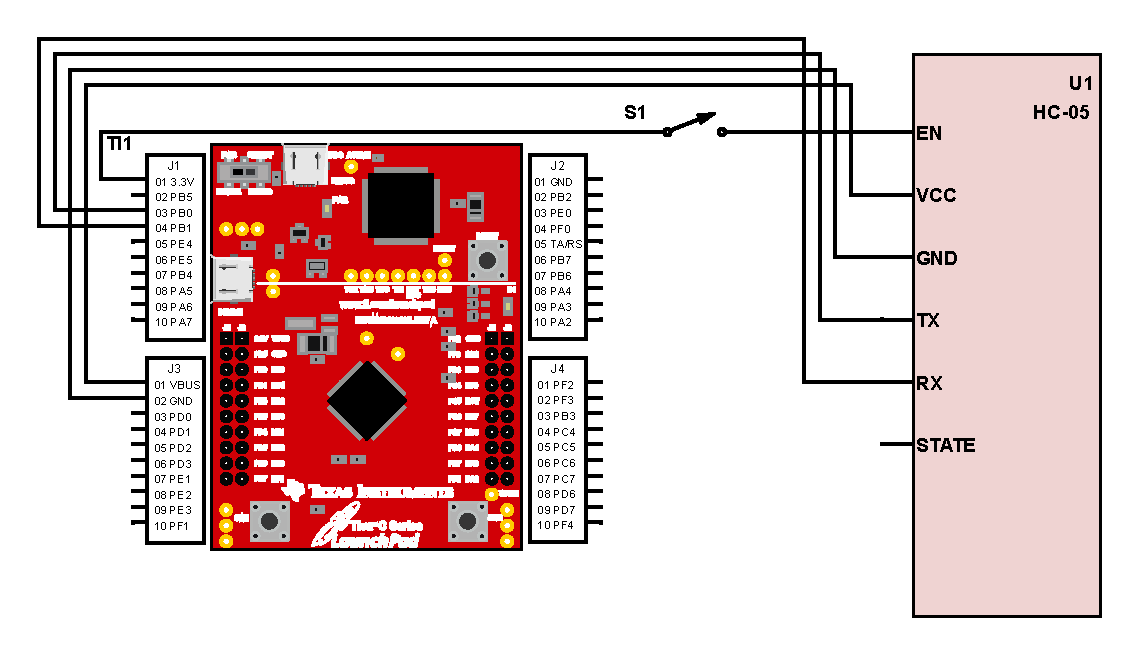
\includegraphics[width=\textwidth]{Images/schemeit-project}
	\caption{The schematic diagram for the Project.}
	\label{schematic}
\end{figure}

\begin{figure}[H]
	\centering
	\includegraphics[width=\textwidth]{"Images/20211211_175133"}
	\caption{Picture of embedded system in action.}
	\label{pic}
\end{figure}

\section{Software Design}
The design for Part 1 was comparatively harder than Part 2.
Part 2's software only consists of setting up the GPIO and
UART modules on the Launchpad for communication with
the HC-05. As I said before, the Launchpad only sees a
UART module, and does not differentiate between a standard
serial terminal or the HC-05.

Part 1's design is a bit harder. It has to check if the
command is correctly formatted before sending it to
the HC-05.

\section{Conclusion}
I had a few issues while making this project such as
my first HC-05 not working due to it having v4 firmware,
but after I got my second HC-05 with v2 firmware and I
bug-tested my code, I was able to complete the project.

\end{document}
